%
%Не забыть:
%--------------------------------------
%Вставить колонтитулы, поменять название на титульнике



%--------------------------------------

\documentclass[a4paper, 12pt]{article} 

%--------------------------------------
%Russian-specific packages
%--------------------------------------
%\usepackage[warn]{mathtext}
\usepackage[T2A]{fontenc}
\usepackage[utf8]{inputenc}
\usepackage[english,russian]{babel}
\usepackage[intlimits]{amsmath}
\usepackage{esint}
%--------------------------------------
%Hyphenation rules
%--------------------------------------
\usepackage{hyphenat}
\hyphenation{ма-те-ма-ти-ка вос-ста-нав-ли-вать}
%--------------------------------------
%Packages
%--------------------------------------
\usepackage{amsmath}
\usepackage{amssymb}
\usepackage{amsfonts}
\usepackage{amsthm}
\usepackage{latexsym}
\usepackage{mathtools}
\usepackage{etoolbox}%Булевые операторы
\usepackage{extsizes}%Выставление произвольного шрифта в \documentclass
\usepackage{geometry}%Разметка листа
\usepackage{indentfirst}
\usepackage{wrapfig}%Создание обтекаемых текстом объектов
\usepackage{fancyhdr}%Создание колонтитулов
\usepackage{setspace}%Настройка интерлиньяжа
\usepackage{lastpage}%Вывод номера последней страницы в документе, \lastpage
\usepackage{soul}%Изменение параметров начертания
\usepackage{hyperref}%Две строчки с настройкой гиперссылок внутри получаеммого
\usepackage[usenames,dvipsnames,svgnames,table,rgb]{xcolor}% pdf-документа
\usepackage{multicol}%Позволяет писать текст в несколько колонок
\usepackage{cite}%Работа с библиографией
\usepackage{subfigure}% Человеческая вставка нескольких картинок
\usepackage{tikz}%Рисование рисунков
\usepackage{float}% Возможность ставить H в положениях картинки
% Для картинок Моти
\usepackage{misccorr}
\usepackage{lscape}
\usepackage{cmap}



\usepackage{graphicx,xcolor}
\graphicspath{{Pictures/}}
\DeclareGraphicsExtensions{.pdf,.png,.jpg}

%----------------------------------------
%Список окружений
%----------------------------------------
\newenvironment {theor}[2]
{\smallskip \par \textbf{#1.} \textit{#2}  \par $\blacktriangleleft$}
{\flushright{$\blacktriangleright$} \medskip \par} %лемма/теорема с доказательством
\newenvironment {proofn}
{\par $\blacktriangleleft$}
{$\blacktriangleright$ \par} %доказательство
%----------------------------------------
%Список команд
%----------------------------------------
\newcommand{\grad}
{\mathop{\mathrm{grad}}\nolimits\,} %градиент

\newcommand{\diver}
{\mathop{\mathrm{div}}\nolimits\,} %дивергенция

\newcommand{\rot}
{\ensuremath{\mathrm{rot}}\,}

\newcommand{\Def}[1]
{\underline{\textbf{#1}}} %определение

\newcommand{\RN}[1]
{\MakeUppercase{\romannumeral #1}} %римские цифры

\newcommand {\theornp}[2]
{\textbf{#1.} \textit{ #2} \par} %Написание леммы/теоремы без доказательства

\newcommand{\qrq}
{\ensuremath{\quad \Rightarrow \quad}} %Человеческий знак следствия

\newcommand{\qlrq}
{\ensuremath{\quad \Leftrightarrow \quad}} %Человеческий знак равносильности

\renewcommand{\phi}{\varphi} %Нормальный знак фи

\newcommand{\me}
{\ensuremath{\mathbb{E}}}

\newcommand{\md}
{\ensuremath{\mathbb{D}}}



%\renewcommand{\vec}{\overline}




%----------------------------------------
%Разметка листа
%----------------------------------------
\geometry{top = 3cm}
\geometry{bottom = 2cm}
\geometry{left = 1.5cm}
\geometry{right = 1.5cm}
%----------------------------------------
%Колонтитулы
%----------------------------------------
\pagestyle{fancy}%Создание колонтитулов
\fancyhead{}
%\fancyfoot{}
\fancyhead[R]{\textsc{Получение и измерение вакуума}}%Вставить колонтитул сюда
%----------------------------------------
%Интерлиньяж (расстояния между строчками)
%----------------------------------------
%\onehalfspacing -- интерлиньяж 1.5
%\doublespacing -- интерлиньяж 2
%----------------------------------------
%Настройка гиперссылок
%----------------------------------------
\hypersetup{				% Гиперссылки
	unicode=true,           % русские буквы в раздела PDF
	pdftitle={Заголовок},   % Заголовок
	pdfauthor={Автор},      % Автор
	pdfsubject={Тема},      % Тема
	pdfcreator={Создатель}, % Создатель
	pdfproducer={Производитель}, % Производитель
	pdfkeywords={keyword1} {key2} {key3}, % Ключевые слова
	colorlinks=true,       	% false: ссылки в рамках; true: цветные ссылки
	linkcolor=blue,          % внутренние ссылки
	citecolor=blue,        % на библиографию
	filecolor=magenta,      % на файлы
	urlcolor=cyan           % на URL
}
%----------------------------------------
%Работа с библиографией (как бич)
%----------------------------------------
\renewcommand{\refname}{Список литературы}%Изменение названия списка литературы для article
%\renewcommand{\bibname}{Список литературы}%Изменение названия списка литературы для book и report
%----------------------------------------
\begin{document}
	\begin{titlepage}
		\begin{center}
			$$$$
			$$$$
			$$$$
			$$$$
			% To be reworked
			{\Large{НАЦИОНАЛЬНЫЙ ИССЛЕДОВАТЕЛЬСКИЙ УНИВЕРСИТЕТ}}\\
			\vspace{0.1cm}
			{\Large{ВЫСШАЯ ШКОЛА ЭКОНОМИКИ}}\\
			\vspace{0.25cm}
			{\large{Факультет физики}}\\
			\vspace{4cm}
			{\Huge\textbf{{Лабораторная работа}}}\\%Общее название
			\vspace{1cm}
			{\LARGE{<<Получение и измерение вакуума>>}}\\%Точное название
			\vspace{2cm}
			{Работу выполнила группа студентов 3 курса}\\
			{Захаров Сергей Дмитриевич \\
			Иевлева Валерия Андреевна\\
			Лопатина Софья Алексеевна}
			\vfill
			%\begin{figure}[H]
			%	\centering
			%	\subfigure{
			%	
\includegraphics[width = 0.2\textwidth]{HSElogo}}
			%	\hspace{4cm}
			%	\subfigure{
			%	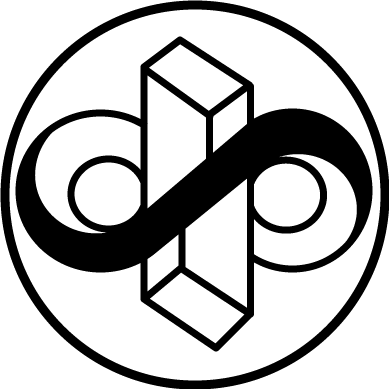
\includegraphics[width = 0.2\textwidth]{IITPlogo}
			%}
			%\end{figure}
			
\includegraphics[width=0.2\linewidth]{HSElogo}
			\vfill
			Москва\\
			2020
		\end{center}
	\end{titlepage}

\tableofcontents

\section{Цель работы}

Перед выполнением работы были поставлены следующие цели:

\begin{enumerate}
	\item Получить вакуум с помощью форвакуумного и цеолитового насосов, и определить динамику его создания.
	
	\item Определить скорость откачки форвакуумного и цеолитового насосов спустя 15 секунд после начала их работы.
\end{enumerate}

\section{Теоретическое введение}

Для определения скорости откачки воспользуемся определением этой физической величины:

\begin{equation}
	S := \left(\frac{dV}{dt}\right)_p
	\label{eq:speed_def}
\end{equation}

Понятно, что подобное определение, строго говоря, в реальности имеет смысл только в каждый отдельно взятый момент времени, поскольку давление постоянно уменьшается в результате работы насоса.

Предположим, что газ, который откачивается из вакуумной камеры, -- идеальный, а процесс происходит при постоянной температуре. В таком случае возможно использование закона Бойля-Мариотта (в приращениях):

\begin{equation*}
	pV = (p + dp) \cdot (V + dV)
	\label{eq:Boil}
\end{equation*}

Раскроем скобки и пренебрежем членом второй степени малости $dp \; dV$:

\begin{equation*}
	dV = -V \frac{dp}{p} = -V d (\ln p) \qrq \frac{dV}{dt} \stackrel{\text{def}}{=} S = -V \frac{d(\ln p)}{dt}
\end{equation*}

Учтем также следующее:

\begin{equation*}
	-d (\ln p) = d (\ln p_0 - \ln p) = d \ln \frac{p_0}{p}
\end{equation*}

В таком случае из вышеуказанного получаем:

\begin{equation}
	S = V \frac{d[\ln (p_0/p)]}{dt}
	\label{eq:speed_use}
\end{equation}

\section{Ход работы}

\subsection{Форвакуумный насос}
\label{sc:foreline}

Во время откачки газа из вакуумной камеры были получены значения давления внутри камеры в последовательные моменты времени, которые приведены на рисунке (\ref{fig:oil_p}). На основании этого графика возможно построить график величины $\ln (p_0/p)$, который представлен на рисунке (\ref{fig:oil_ln}). После этого, с помощью последнего графика, возможно с помощью формулы (\ref{eq:speed_use}) определить скорость откачки насоса в момент времени $t=15$~с. Если принять $V\approx 3.45$~л, то получаем значение $\boxed{S_{fl} \approx 0.056\text{ л/с}}$.

\begin{figure}[h]
	\centering
	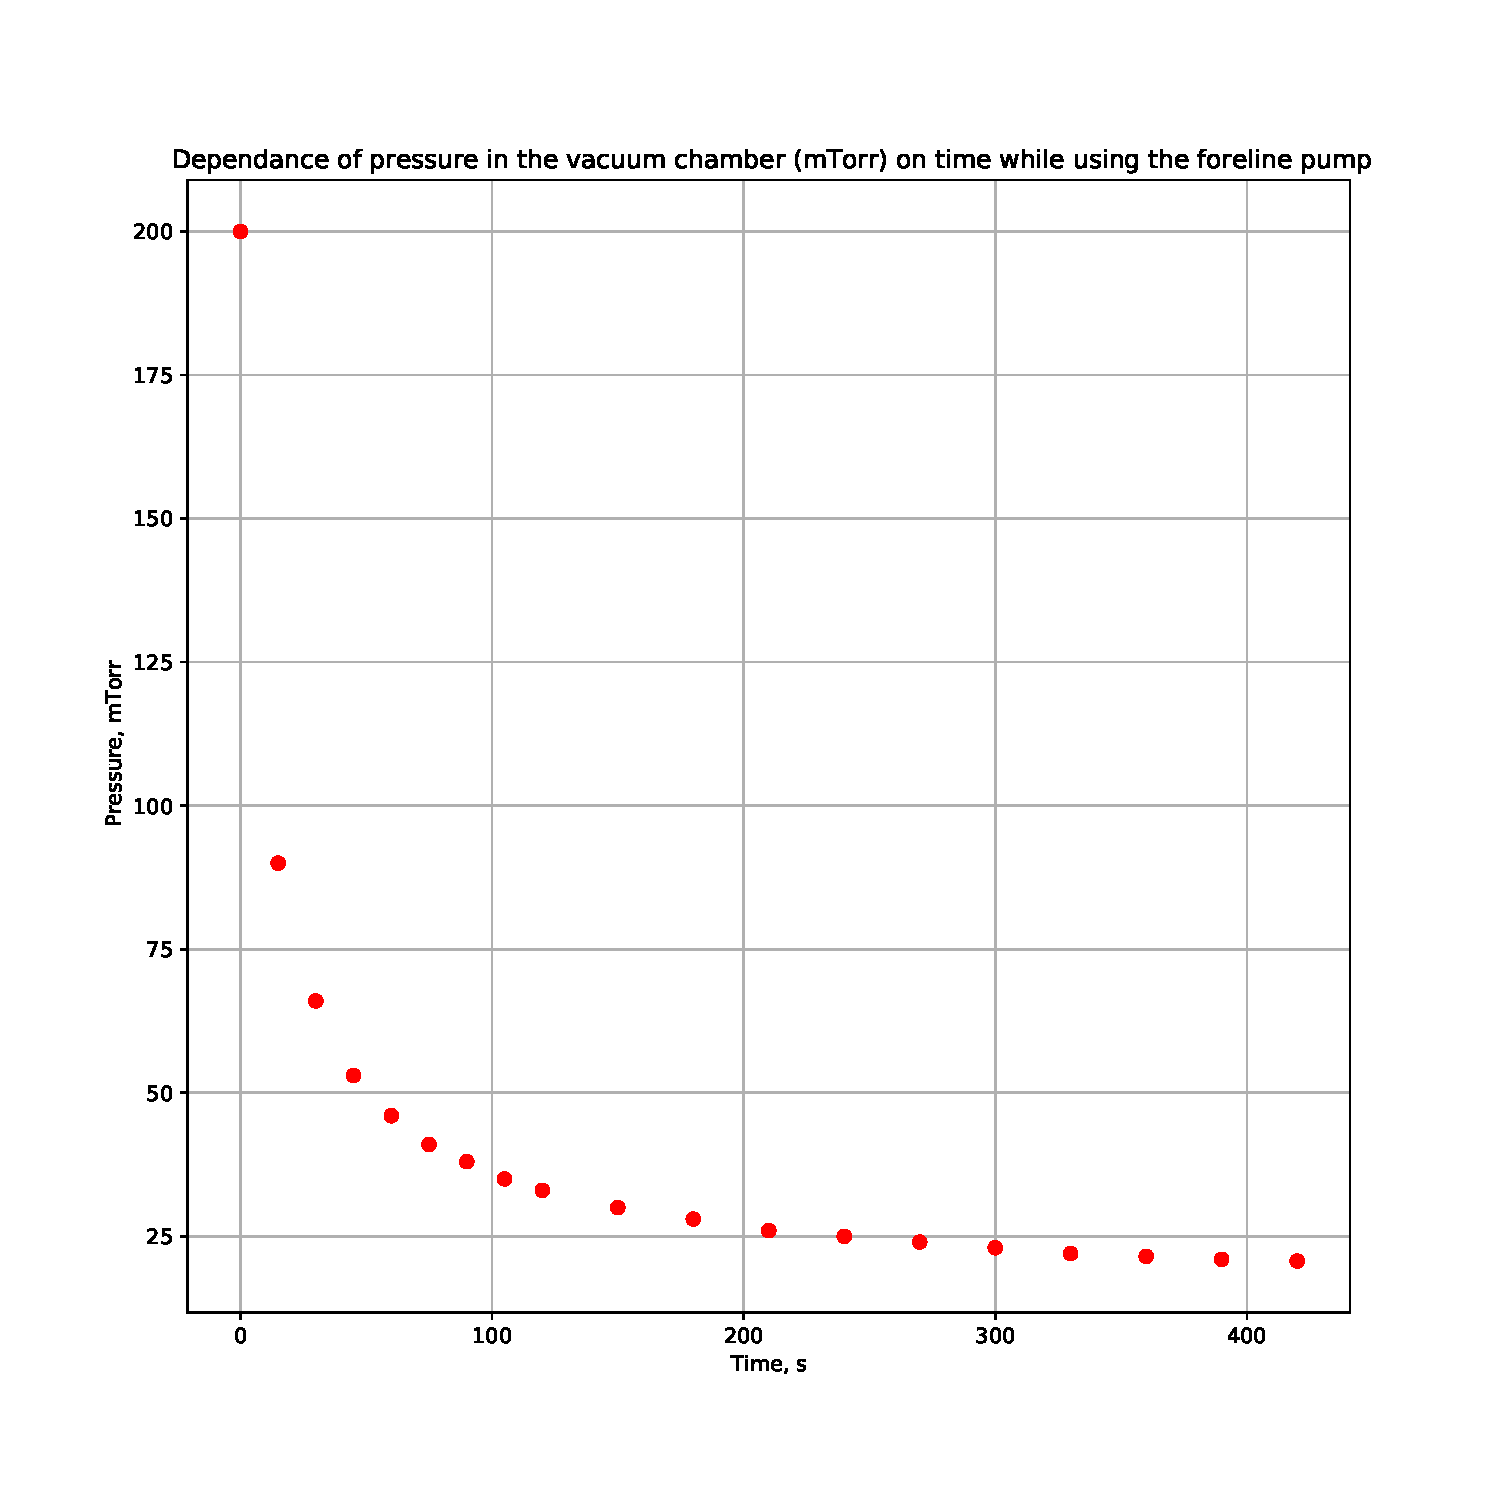
\includegraphics[width=0.8\linewidth]{lab_1_oil_p}
	\caption{Зависимость давления внутри вакуумной камеры от времени при использовании форвакуумного насоса.}
	\label{fig:oil_p}
\end{figure}

\begin{figure}[h]
	\centering
	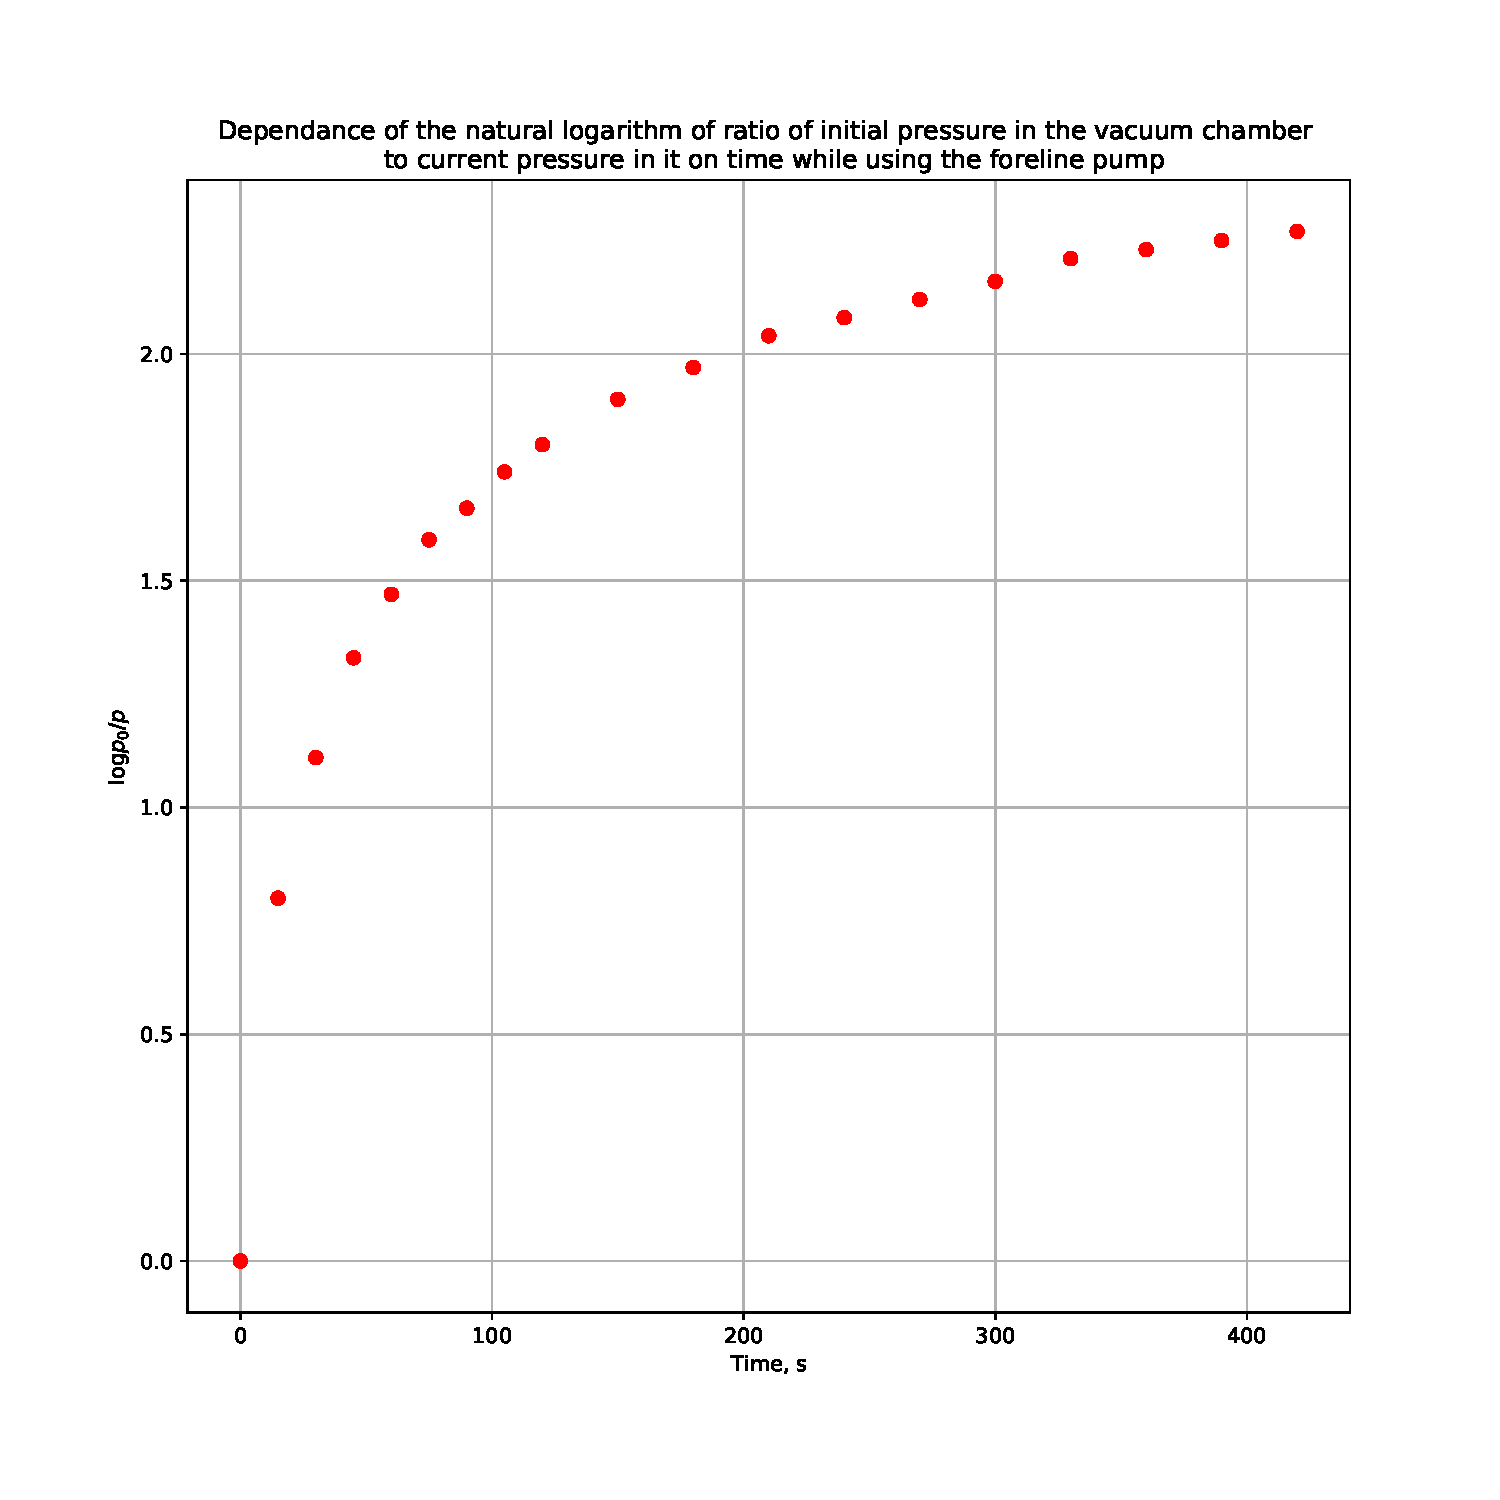
\includegraphics[width=0.8\linewidth]{lab_1_oil_ln}
	\caption{Зависимость натурального логарифма отношения давления в вакуумной камере в начальный момент времени к текущему давлению в ней от времени при использовании форвакуумного насоса.}
	\label{fig:oil_ln}
\end{figure}

\subsection{Цеолитовый насос}

Метод выполнения работы совпадает с уже описанном в разделе \nameref{sc:foreline}, поэтому здесь приведем только полученные графики, которые указаны на рисунках (\ref{fig:cryo_p}) и (\ref{fig:cryo_ln}), а также полученное значение скорости откачки: $\boxed{S_{ze} = 0.051 \text{ л/с}}$.

\begin{figure}[h]
	\centering
	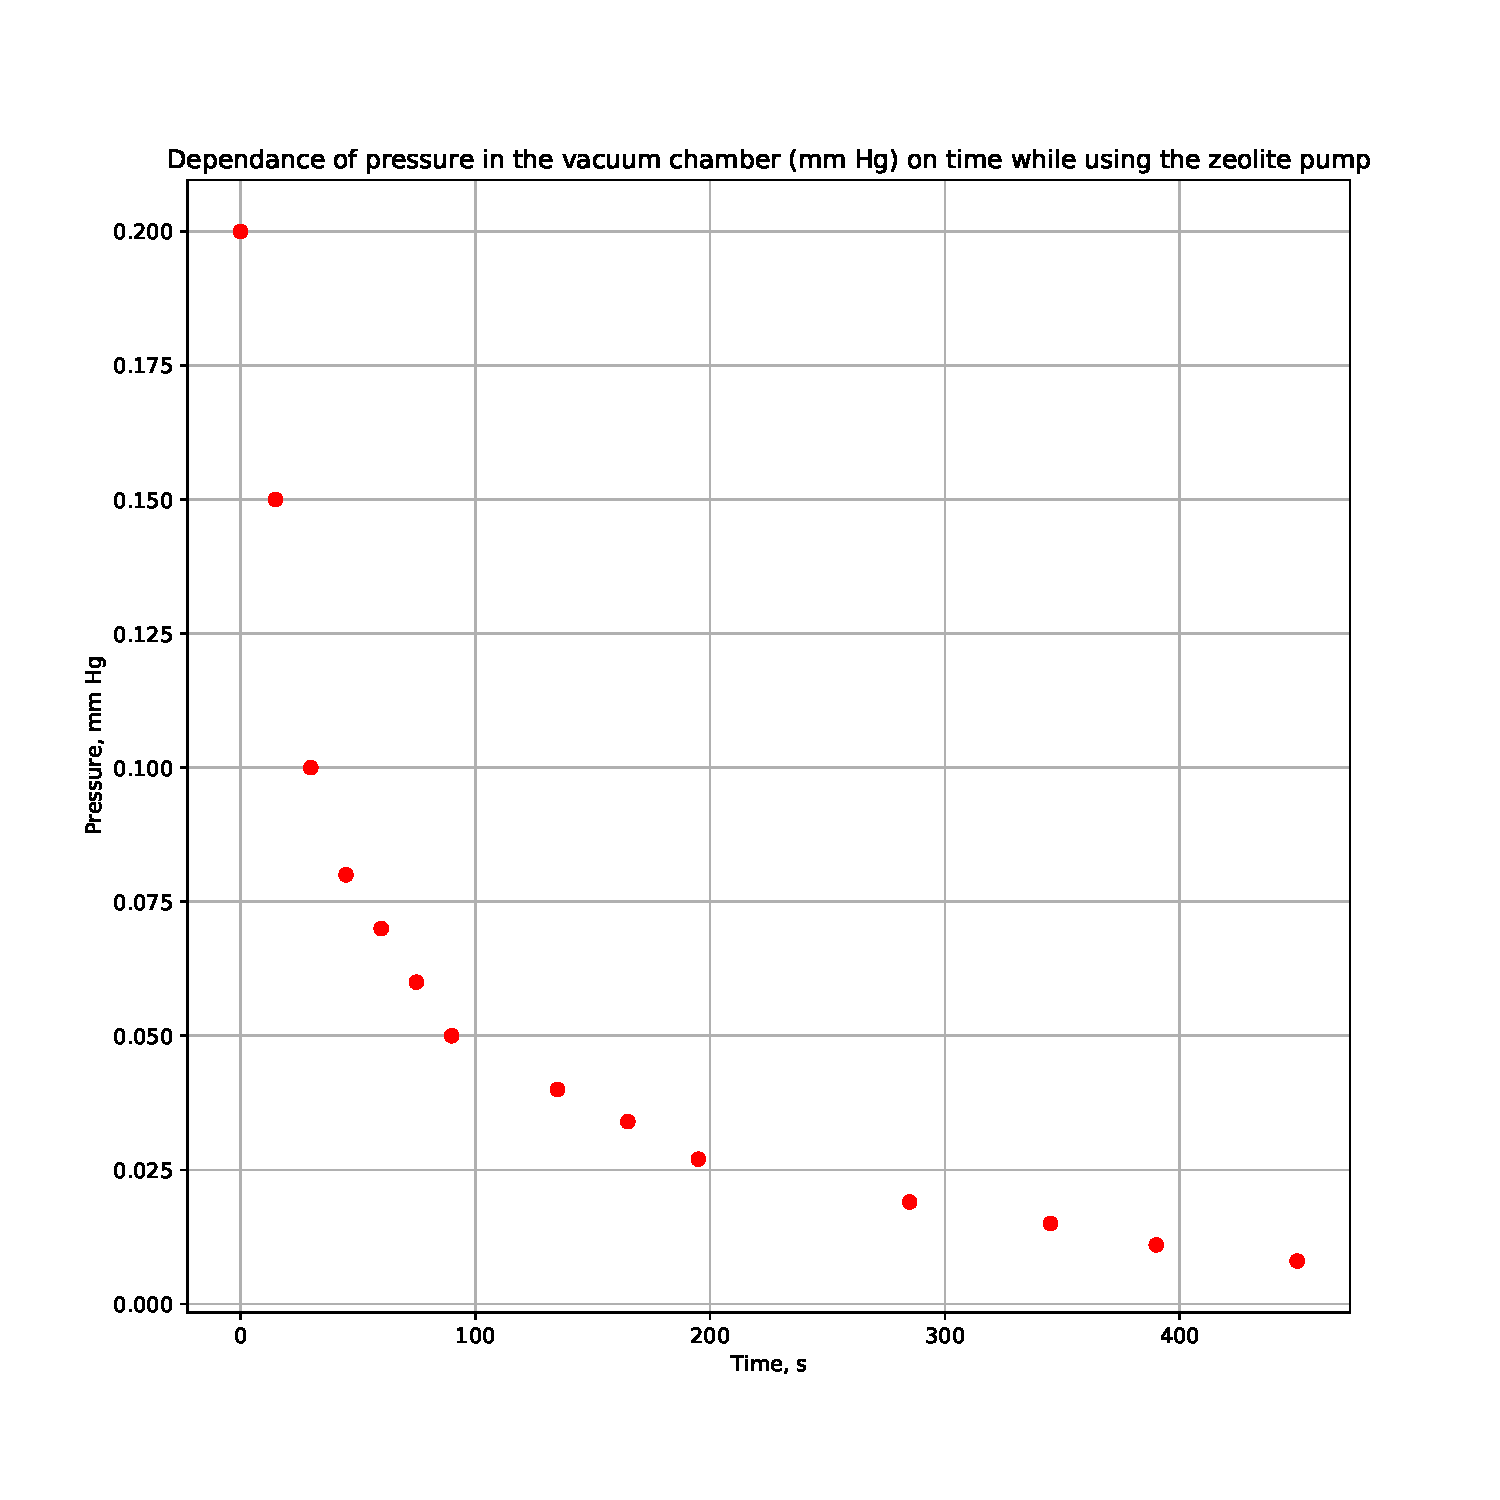
\includegraphics[width=0.8\linewidth]{lab_1_cryo_p}
	\caption{Зависимость давления внутри вакуумной камеры от времени при использовании цеолитового насоса.}
	\label{fig:cryo_p}
\end{figure}

\begin{figure}[h]
	\centering
	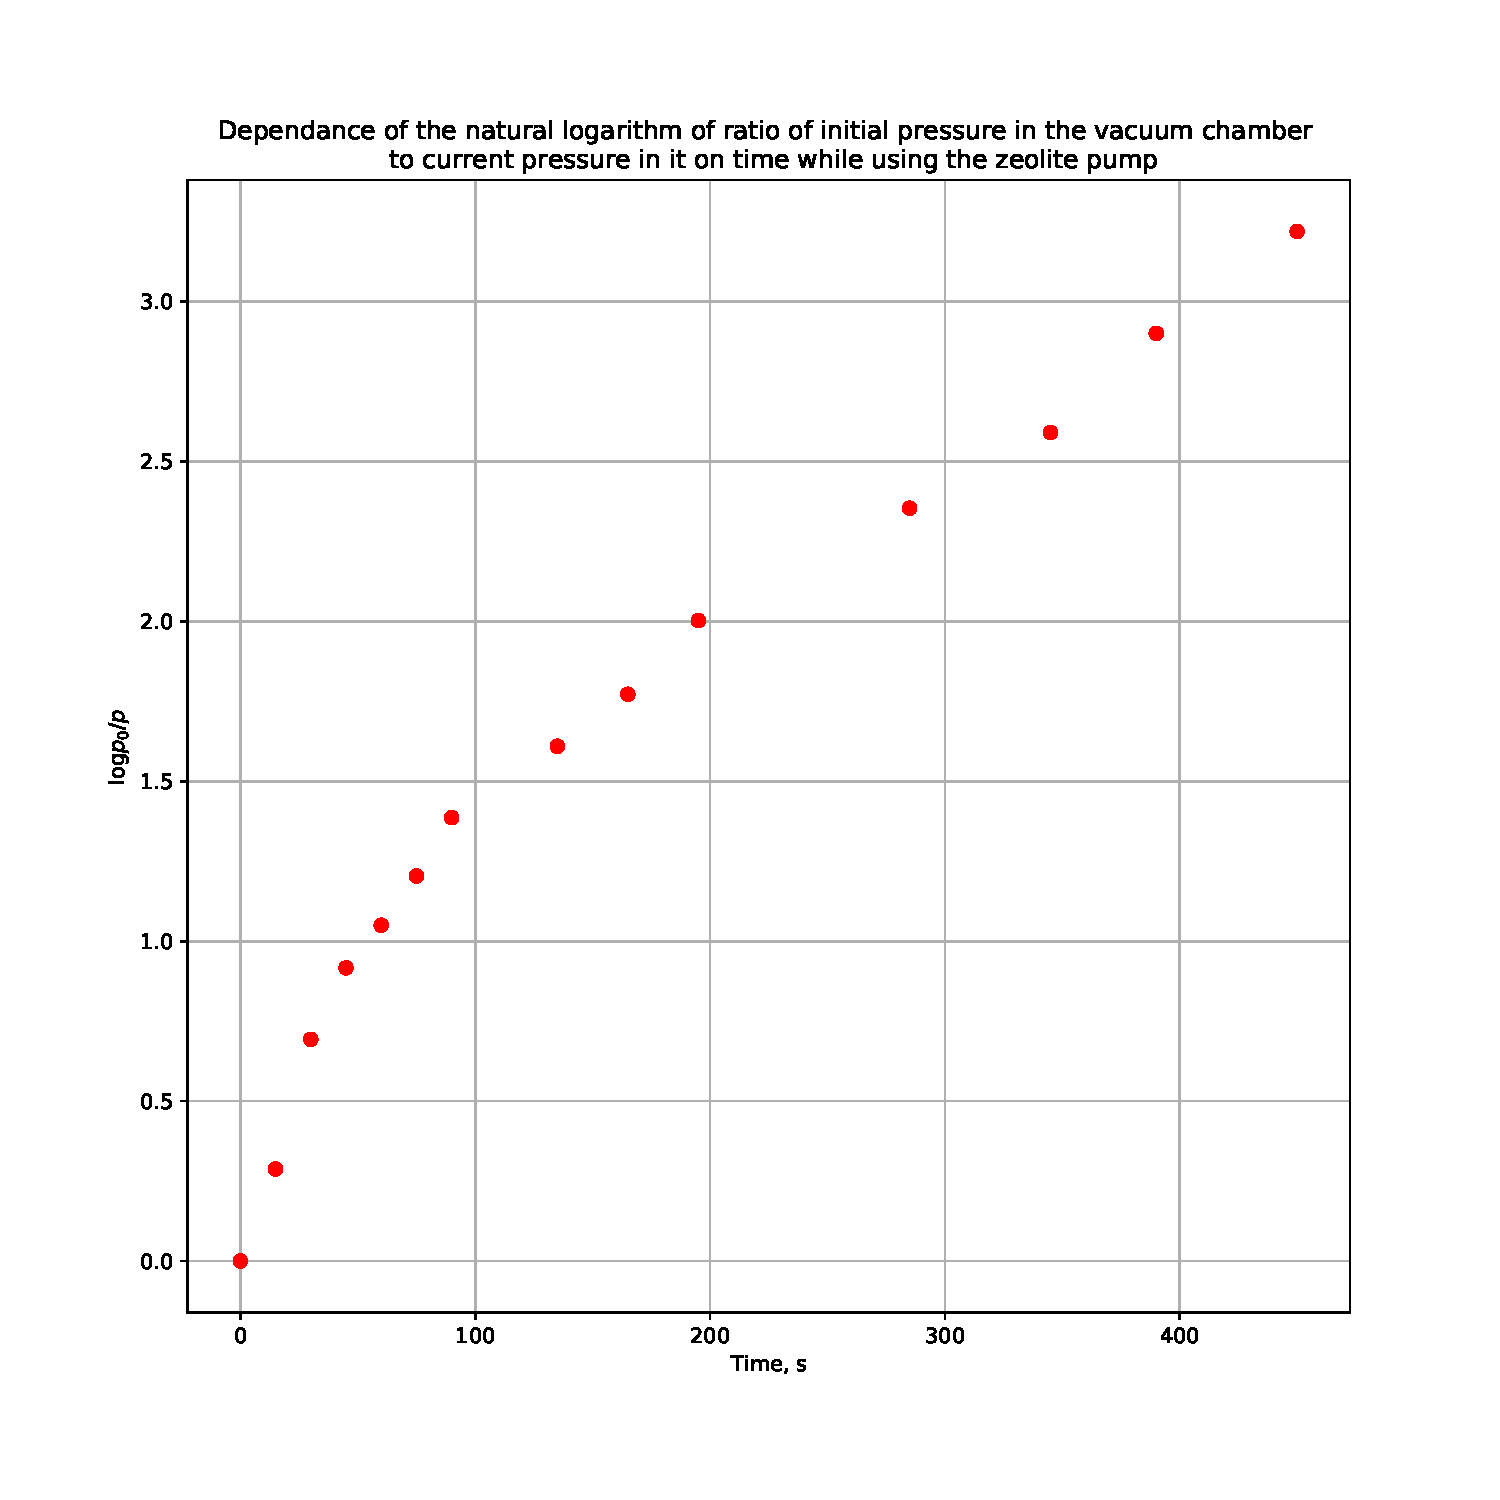
\includegraphics[width=0.8\linewidth]{lab_1_cryo_ln}
	\caption{Зависимость натурального логарифма отношения давления в вакуумной камере в начальный момент времени к текущему давлению в ней от времени при использовании цеолитового насоса.}
	\label{fig:cryo_ln}
\end{figure}

\section{Вывод}

\begin{enumerate}
	\item В результате работы были определены зависимости давления в вакуумной камере от времени при использовании насосов двух типов: форвакуумного и цеолитового.
	
	\item Были определены скорости откачки указанных насосов в момент времени $t=15$~с: $\boxed{S_{fl} \approx 0.056\text{ л/с}}$, $\boxed{S_{ze} = 0.051 \text{ л/с}}$.
\end{enumerate}








\end{document}